%File: formatting-instruction.tex
\documentclass[letterpaper]{article}
\usepackage{aaai}
\usepackage{times}
\usepackage{helvet}
\usepackage{courier}
\usepackage{graphicx}

\usepackage{listings}


\frenchspacing
\setlength{\pdfpagewidth}{8.5in}
\setlength{\pdfpageheight}{11in}
\pdfinfo{
/Title (Plan Scheduling: Managing story coherence for cinematic camera control)
/Author (Put All Your Authors Here, Separated by Commas)}
\setcounter{secnumdepth}{0}  
 \begin{document}
% The file aaai.sty is the style file for AAAI Press 
% proceedings, working notes, and technical reports.
%
\title{Plan Scheduling: A Plan-based Approach to Managing Story Coherence \break For Cinematic Camera Control}
\author{David R. Winer\\
School of Computing\\
2275 East Bayshore Road, Suite 160\\
Palo Alto, California 94303\\
}
\maketitle
\begin{abstract}
\begin{quote}
AAAI creates proceedings, working notes, and technical reports directly from electronic source furnished by the authors. To ensure that all papers in the publication have a uniform appearance, authors must adhere to the following instructions. 
\end{quote}
\end{abstract}

\noindent
The role of a film director is to design and create the scenes of a film. The task involves directing characters and planning out visual details across camera shots. Film directing is a very large logistical challenge, and AI tools have the potential to make this process easier. Film directors can prototype ideas for a scene using a game engine, and receive recommendations by using patterns extracted from existing film productions. 

One of the primary challenges that AI can alleviate for scene directing is managing coherence. Coherence refers to the structural properties of a film that are designed to help a viewer piece together a story from individual camera shots. We focus on three dimensions of coherence:
\begin{enumerate}
    \item Story Coherence - changes in a world state are explained, and there is a logical flow of events from the initial state to the final state.
    \item Frame Coherence - transitions between shots enable story-focused attention and avoid disorienting viewers.
    \item Communicative Coherence - a communicative action is interpreted with its desired meaning. See Figure \ref{fig:bondsequence} for a cinematic example.
\end{enumerate}

\begin{figure}[b]
    \centering
    \includegraphics{}
    \caption{Caption}
    \label{fig:bondsequence}
\end{figure}

An AI scene director is a system that constructs a camera schedule for creating a scene. The goal of a scene directing system is to produce a schedule that manages story coherence and achieves a set of communicative goals. The schedule represents a timeline of camera actions for cinematic camera control. Each action represents a camera shot or shot sequence and can reference intervals of the storyworld in any order. The execution of the actions in the schedule represent camera instructions for filming the referenced storyworld interval. We focus on two kinds of shot sequence:

\begin{itemize}
    \item Goal-driven camera sequence: a shot or shot sequence focused on a specific communicative goal.
    \item Goal-agnostic camera sequence: a shot or shot sequence focused on frame coherence and not on a specific communicative goal.
\end{itemize}


One previous approach that used goal-driven camera sequences in scene directing is Darshak \cite{jhala2010cinematic}. Darshak receives communicative goals as input, operator schemata for goal-driven camera sequences, and a complete story plan. Darhsak's camera planning module finds instances of the story that fit the constraint patterns defined in camera sequence templates that are in support of its communicative goals. Like most camera planning modules, it cannot modify or add to the story, and doing so can affect story coherence. One of the limitations is that the expressiveness of camera sequence story patterns is limited to what the sequence template designer can predict is in the story. A scene director should have fine-grain control over the story. Film directors achieve fine-grain control by combining story directing and camera planning into the same reasoning process. 

Another approach by \citeauthor{galvane2015continuity} (\citeyear{galvane2015continuity}) is to focus on goal-agnostic camera sequences. They use a formula to aggregate various dimensions of frame coherence including motion continuity, gaze continuity, left-to-right ordering, and others into a single measure. Given an immutable story, a finite set of cameras, and a finite set of moments, they find the camera sequence that maximizes frame coherence between adjacent shots.

Plan-based methods are useful for managing story coherence \cite{riedl2010narrative,young2013plans}. However, there are currently two main limitations to using a plan-based method for constructing a film schedule. First, cinematic sequences may appear inefficient when compared to a plan optimized to solve a planning problem. This is because there is a disconnect between the efficient behavior one would see in a plan-driven agent and the behavior one would see in a cinematic sequence created by a human director. A plan-based approach needs to manage this inefficiency while not deviating from the task of managing story coherence. Second, cinematic discourse consists of two fundamental kinds of plans that are interrelated: one kind of plan representing the story and another representing the camera schedule. This is similar to the way narratologists distinguish story and discourse \cite{chatman1980story,genette1983narrative,young2007story,bordwell2013narration}. Previous approaches have not combined reasoning about two kinds of plans in this way.

Our approach to scene directing uses a novel planning framework to combine story and camera reasoning. The approach is called \textit{plan scheduling} and refers to the task of constructing a story plan and a camera schedule so that the story is coherent and the camera schedule achieves any communicative goals that are provided as input. A high-level depiction of the task is given in Figure \ref{fig:planscheduling}. The framework overcomes limitations of previous plan-based approaches to cinematic camera control by rewarding the planner for using cinematic sequences and solving challenges for maintaining story coherence. 

\begin{figure}
    \centering
    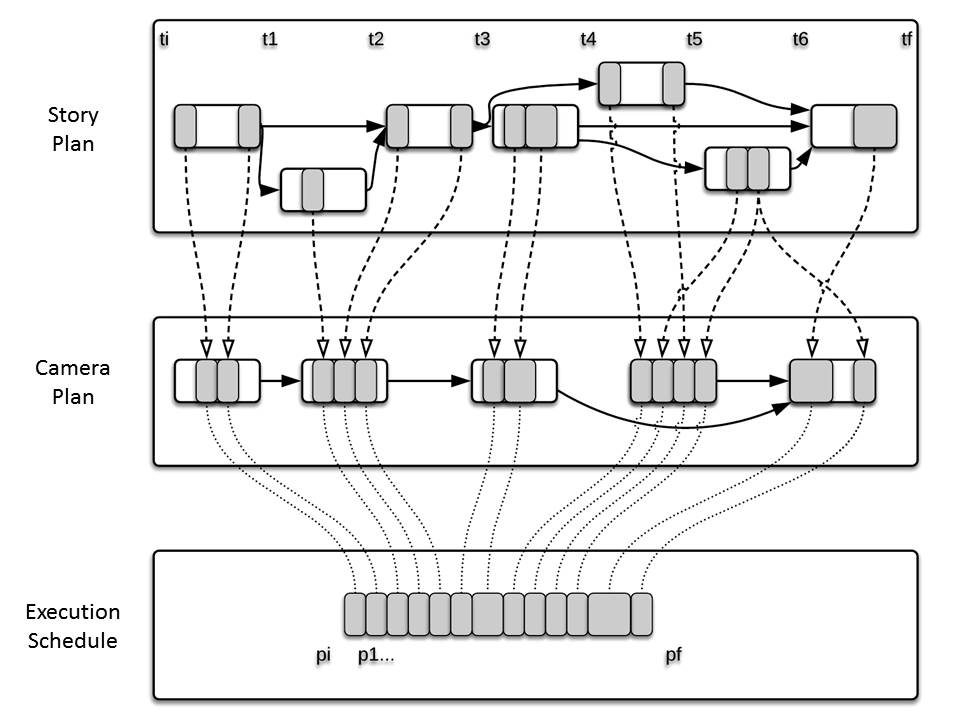
\includegraphics[scale=0.34]{PlanScheduling.jpg}
    \caption{A high-level depiction of the plan scheduling task. The top row is the story plan which should be coherent (i.e. executable). The middle row is a camera plan whose actions are shots or shot sequences that reference intervals of story actions in any order. The final scene execution is just the execution of the story action intervals in the order referenced in the camera plan.}
    \label{fig:planscheduling}
\end{figure}

\paragraph{Contributions}: A planning and scheduling framework for scene directing, and an extension that leverages a film scene directing knowledge representation.

\section{Related Work}

\subsection{Story Coherence}

\subsection{Cinematic Camera Control}


% in order to leverage goal-agnostic and goal-driven camera sequences in its output schedule while maintaining story coherence. 

%  The final execution of the world is just the execution of the intervals of the storyworld in the order they are referenced in the schedule. .
\subsection{Plan-space Planning}

Our approach extends an AI planning technique. Here, we give some background on the foundation our approach uses. 

A world state is a conjunction of first-order literals that describe conditions of the world as true or false. An operator template is a schema for explaining changes in a world state. A task for a planner is a planning problem. It contains the operator templates, a set of typed objects, an initial world state, and a set of goal conditions that need to be explained. The task is solved by a plan if the execution of the plan transitions the initial state into a state consistent with the goal conditions.

Different kinds of planners perform different kinds of search. Our planning work extends plan-space search. In a plan-space search, each node represents a partial plan, and each edge represents a repair to an inconsistency in the parent node. The leaves of the tree are either solutions (i.e. whole plans), or partial plans with inconsistencies that cannot be repaired. Specifically, we build on partial-order causal link (POCL) planning \cite{penberthy1992ucpop,weld1994introduction}, which searches in the space of plans to find a partial plan (i.e. a set of steps $S$, a set of partial ordering relations $O$ over $S$, and a set of causal links $L$) with no \emph{flaws}; all preconditions must be satisfied (no condition may remain \emph{open}) and no causal links may be \emph{threatened} (i.e. it should not be possible for any step to be ordered such that it potentially undoes a causal link's protected literal). Open conditions are repaired through \emph{adding} or \emph{reusing} a plan step and threatened causal links are repaired by \emph{promoting} or \emph{demoting} the offending step to come after or before (respectively) the threatened link. For a more thorough introduction to POCL planning, we refer the reader to \citeA{weld1994introduction}. 

Our approach extends decompositional planning. In decompositional planning, a composite (i.e. abstract) action cannot execute directly in a plan. Instead, it must decompose into a sub-plan whose sub-steps can either execute directly or decompose further. The formal model of decompositional planning we adopt is taken from DPOCL, a planning system previously developed by \cite{young1994decomposition}. DPOCL has two kinds of steps. A \emph{primitive step} is as in POCL planning, and a \textit{composite step} is a step that is decomposable into a partial-plan, called a \textit{sub-plan}. Each composite step is a composite operator type paired with a set of bindings over operator parameters. In this paper, composite steps are associated with a single decomposition method and a set of bindings over decomposition parameters (i.e. a composite operator is rewritten with a specific decomposition method). A step in the sub-plan of a composite step is a \textit{sub-step}. The decomposition specifies constraints over partially defined sub-steps that are useful in our application. A \textit{decompositional link} relates a composite step to a sub-step. The \textit{height} of a composite step is the longest path of decomposition links. Thus a decompositional plan is represented by a tuple $\langle S, O, L, D \rangle$ where $D$ is a set of decompositional links. 


\section{Plan Scheduling}

Plan scheduling is an extension of decompositional planning where composite actions are used to represent cinematic sequences. Whereas composite actions are typically efficiency hacks, saving the planner on the iterations it would take to add its sub-steps individually and make repairs. However, cinematic sequences may be inefficient with respect to solving a planning problem. To use cinematic sequences in its output, a planner needs to allow some inefficiency while not deviating from the central task of solving the planning problem. Previous work has leveraged ground composite actions to enable heuristic estimates that 

Also, composite actions are used to add both story actions and camera actions. Whereas previous plan-based approaches use an immutable story plan as input (e.g. Storybook cite(callaway),\cite{jhala2010cinematic}), our approach is 

Plan scheduling solves two major limitations to using a plan-based approach story coherence in a cinematic camera control task. The first challenge is that cinematic sequences 

The first challenge is representing the task, and the second challenge is that cinemati. Composite actions represent cinematic sequences that decompose into the story actions needed in the sequence and the 

 To address this challenge we add a reward function that motivates the use of composite actions. representing cinematic sequences.

A primitive action is ground if each parameter variable is assigned a problem object. A composite action is ground if each sub-step in its sub-plan is ground and each parameter variable is assigned a problem object. A problem is ground if it contains the complete set of ground actions. Ground Decompositional Partial Order Planning (GDPOP) solves a planning problem by adding and reusing ground composite actions. GDPOP can leverage that composite actions are ground when calculating heuristic estimates. 

\section{Film Directing Task}





\section{Plan Scheduling}

\section{Cinematic Directing}


\bibliography{aaai}
\bibliographystyle{aaai}
\end{document}